%\documentclass[portrait,final,a0paper,fontscale=0.385]{baposter}
\documentclass[portrait,final,a0paper,fontscale=0.38]{baposter}

\usepackage{calc}
\usepackage{graphicx}
\usepackage{amssymb}
\usepackage{relsize}
\usepackage{multirow}
\usepackage{rotating}
\usepackage{bm}
\usepackage{url}

\usepackage{amsfonts,amsmath, amsthm}

\newtheorem{proposition}{Proposition}


\usepackage{color}
\usepackage[utf8]{inputenc}
\usepackage[T1]{fontenc}
\usepackage{fancyhdr}
\usepackage{color}
\usepackage{fancybox}
\usepackage{epsfig}
\usepackage{array}

\usepackage{multicol}
\usepackage{float}
%\usepackage{times}
%\usepackage{helvet}
%\usepackage{bookman}
\usepackage{palatino}
\usepackage{subfig}

\usepackage{wrapfig}

\renewcommand*\familydefault{\sfdefault} %% Only if the base font of the document is to be sans serif

\graphicspath{{images/}{../images/}}
\usetikzlibrary{calc}


%%%%%%%%%%%%%%%%%%%%%%%%%%%%%%%%%%%%%%%%%%%%%%%%%%%%%%%%%%%%%%%%%%%%%%%%%%%%%%%%
%%%% Some math symbols used in the text
%%%%%%%%%%%%%%%%%%%%%%%%%%%%%%%%%%%%%%%%%%%%%%%%%%%%%%%%%%%%%%%%%%%%%%%%%%%%%%%%

%%%%%%%%%%%%%%%%%%%%%%%%%%%%%%%%%%%%%%%%%%%%%%%%%%%%%%%%%%%%%%%%%%%%%%%%%%%%%%%%
% Multicol Settings
%%%%%%%%%%%%%%%%%%%%%%%%%%%%%%%%%%%%%%%%%%%%%%%%%%%%%%%%%%%%%%%%%%%%%%%%%%%%%%%%
\setlength{\columnsep}{1.5em}
\setlength{\columnseprule}{0mm}

%%%%%%%%%%%%%%%%%%%%%%%%%%%%%%%%%%%%%%%%%%%%%%%%%%%%%%%%%%%%%%%%%%%%%%%%%%%%%%%%
% Save space in lists. Use this after the opening of the list
%%%%%%%%%%%%%%%%%%%%%%%%%%%%%%%%%%%%%%%%%%%%%%%%%%%%%%%%%%%%%%%%%%%%%%%%%%%%%%%%
\newcommand{\compresslist}{%
\setlength{\itemsep}{0pt}%
\setlength{\parskip}{2pt}%
\setlength{\parsep}{0pt}%
}

%%%%%%%%%%%%%%%%%%%%%%%%%%%%%%%%%%%%%%%%%%%%%%%%%%%%%%%%%%%%%%%%%%%%%%%%%%%%%%
%%% Begin of Document
%%%%%%%%%%%%%%%%%%%%%%%%%%%%%%%%%%%%%%%%%%%%%%%%%%%%%%%%%%%%%%%%%%%%%%%%%%%%%%

\begin{document}

%%%%%%%%%%%%%%%%%%%%%%%%%%%%%%%%%%%%%%%%%%%%%%%%%%%%%%%%%%%%%%%%%%%%%%%%%%%%%%
%%% Here starts the poster
%%%---------------------------------------------------------------------------
%%% Format it to your taste with the options
%%%%%%%%%%%%%%%%%%%%%%%%%%%%%%%%%%%%%%%%%%%%%%%%%%%%%%%%%%%%%%%%%%%%%%%%%%%%%%
% Define some colors

%\definecolor{lightblue}{cmyk}{0.83,0.24,0,0.12}
%\definecolor{lightblue}{RGB}{102,178,255}
%\definecolor{darkblue}{RGB}{0,51,102}
%\definecolor{fondo}{RGB}{153,204,255}
%\definecolor{caja}{RGB}{155,190,220}
%\definecolor{burdeos}{RGB}{204,0,102}

\definecolor{lightblue}{RGB}{231,142,20}
\definecolor{darkblue}{RGB}{208,47,0}
\definecolor{fondo}{RGB}{225,225,225}
\definecolor{caja}{RGB}{231,176,118}
\definecolor{burdeos}{RGB}{204,0,102}




\theoremstyle{plain}
\newtheorem{theorem}{Theorem}
\newtheorem{lemma}{Lemma}
\newtheorem{corollary}{Corollary}
\newtheorem{definition}{Definition}
\newtheorem{remark}{Remark}


\newcommand{\diam}[0]{\mathrm{diam}}
\newcommand{\rad}[0]{\mathrm{rad}}
\newcommand{\diminf}[0]{\underline{\dim}_B}
\newcommand{\dimsup}[0]{\overline{\dim}_B}
\renewcommand{\Re}[0]{\mathrm{Re}\ }
\renewcommand{\Im}[0]{\mathrm{Im}\ }
\renewcommand{\H}[0]{\mathbb{H}}

%MORE PACKAGES HERE
\newcommand{\R}[0]{\mathbb{R}}
\newcommand{\C}[0]{\mathbb{C}}
\newcommand{\N}[0]{\mathbb{N}}
\newcommand{\Z}[0]{\mathbb{Z}}
\newcommand{\Q}[0]{\mathbb{Q}}
\newcommand{\K}[0]{\mathbb{K}}
\newcommand{\sgn}[0]{\mathrm{sgn}}
\newcommand{\supp}[0]{\mathrm{supp}}
\newcommand{\prodesc}[2]{\left\langle #1 , #2 \right\rangle}


\tolerance=1
\emergencystretch=\maxdimen
\hyphenpenalty=10000
\hbadness=10000
%%
\begin{poster}%
  % Poster Options
  {
  columns=2,
  % Show grid to help with alignment
  grid=false,
  % Column spacing
  colspacing=1em,
  % Color style
  bgColorOne=white,
  bgColorTwo=fondo,
  borderColor=lightblue,
  headerColorOne=darkblue,
  headerColorTwo=darkblue,
  %headerColorTwo=lightblue,
  headerFontColor=white,
  boxColorOne=white,
  boxColorTwo=caja,
  % Format of textbox
  textborder=rectangle,
  % Format of text header
  eyecatcher=true,
  headerborder=closed,
  headerheight=0.085\textheight,
%  textfont=\sc, An example of changing the text font
  %headershape=roundedright,
  %headershape=roundedleft,
  %headershade=shadelr,
  headerfont=\Large\bf\textsc, %Sans Serif
  textfont={\setlength{\parindent}{1.5em}},
  boxshade=shadetb,
%  background=shade-tb,
  background=shadetb,
  linewidth=1.5pt
  }
  % Eye Catcher
  % University logo
  {
  	
\includegraphics[height=10em]{ugr}
  }
  % Title
  {
  	\medskip
  	{\scalebox{1.4}{\LARGE{\bf\textsc{\textcolor{darkblue}{Orthogonal Polynomials}}}}}\\
    {\LARGE \textsc{\textcolor{darkblue}{Applications and Bivariate Multiple Orthogonality}}}\vspace{3pt}
  }
  % Authors
  {
  	\textsc{\textbf{J. Antonio Villegas}, Lidia Fernández}
  	\\
  	\small{\texttt{(jantoniovr@ugr.es, lidiafr@ugr.es)}}
  	\\
  	\normalsize{Departamento de Matem\'{a}tica Aplicada and Instituto de Matemáticas IMAG, Universidad de Granada.}
  }
  % Faculty logo
  {
  	
\includegraphics[height=3.8em]{IMAG}
    
  	
\includegraphics[height=3.8em]{maeztu}
  }



%%%%%%%%%%%%%%%%%%%%%%%%%%%%%%%%%%%%%%%%%%%%%%%%%%%%%%%%%%%%%%%%%%%%%%%%%%%%%%
%%% Now define the boxes that make up the poster
%%%---------------------------------------------------------------------------
%%% Each box has a name and can be placed absolutely or relatively.
%%% The only inconvenience is that you can only specify a relative position
%%% towards an already declared box. So if you have a box attached to the
%%% bottom, one to the top and a third one which should be in between, you
%%% have to specify the top and bottom boxes before you specify the middle
%%% box.
%%%%%%%%%%%%%%%%%%%%%%%%%%%%%%%%%%%%%%%%%%%%%%%%%%%%%%%%%%%%%%%%%%%%%%%%%%%%%%
    %
    % A coloured circle useful as a bullet with an adjustably strong filling
    \newcommand{\colouredcircle}{%
      \tikz{\useasboundingbox (-0.2em,-0.32em) rectangle(0.2em,0.32em); \draw[draw=black,fill=lightblue,line width=0.03em] (0,0) circle(0.18em);}}

%%%%%%%%%%%%%%%%%%%%%%%%%%%%%%%%%%%%%%%%%%%%%%%%%%%%%%%%%%%%%%%%%%%%%%%%%%%%%%%
%  \headerbox{Motivation}{name=motivation,column=0,row=0,span=3}{
%%%%%%%%%%%%%%%%%%%%%%%%%%%%%%%%%%%%%%%%%%%%%%%%%%%%%%%%%%%%%%%%%%%%%%%%%%%%%%%

\headerbox{\ 1. Introduction to Orthogonal Polynomials}{name=intro,column=0,row=0,span=2}
  {
%%%%%%%%%%%%%%%%%%%%%%%%%%%%%%%%%%%%%%%%%%%%%%%%%%%%%%%%%%%%%%%%%%%%%%%%%%%%%%%

\begin{multicols}{2}

  Orthogonal Polynomials theory is a branch of approximation theory which could be useful in many other research topics as approximation of functions, differential equations, numerical analysis, stochastic processes and even in other sciences like optics. Everybody knows polynomials and orthogonality, however, what are ``orthogonal polynomials''?

  Let us consider $\R[x]$, the vector space of univariate polynomials. As a vector space, we can provide $\R[x]$ with an inner product $\prodesc{\cdot}{\cdot}:\R[x]\times\R[x]\longrightarrow\R$, which it is often defined using integral functionals. This is, given a one-dimensional measure $\mu$, we can define the inner product
  \begin{equation}
    \label{eq:prodesc}
    \prodesc{P}{Q}_\mu:=\int P(x)Q(x)d\mu(x), \ \ \ \forall P,Q\in\R[x]
  \end{equation}
  Thus, using this inner product, two polynomials $P,Q$ are orthogonal if $\prodesc{P}{Q}_\mu = 0$. This motivates the first definition
  \begin{definition}
    Let $\{P_n\}_{n\geq 0}$ be a sucession of polynomials. Then it is a \textbf{Orthogonal Polynomials Sucession} (OPS) if:
    \begin{enumerate}
      \item $\deg(P_n)=0, \ \ n\geq 0$.
      \item $\prodesc{P_n}{P_k}=0, \ \ 0\geq k < n, n\geq 0$.
      \item $\prodesc{P_n}{P_n} \not = 0, \ \ \ n\geq 0$.
    \end{enumerate}
  \end{definition}
  Then, an OPS shapes a orthogonal basis of $\R[x]$. You can build the OPS from the measure using many different ways: applying Gram-Schmidt orthogonalization process to the usual basis $\{1,x,x^2,\dots\}$, solving linear systems of equations, or applying other proper methods like the Three Term Relation or Rodrigues Formula for the so called `classic' orthogonal polynomials. 


\end{multicols}
%%%%%%%%%%%%%%%%%%%%%%%%%%%%%%%%%%%%%%%%%%%%%%%%%%%%%%%%%%%%%%%%%%%%%%%%%%%%%%%
	}
%%%%%%%%%%%%%%%%%%%%%%%%%%%%%%%%%%%%%%%%%%%%%%%%%%%%%%%%%%%%%%%%%%%%%%%%%%%%%%%


%%%%%%%%%%%%%%%%%%%%%%%%%%%%%%%%%%%%%%%%%%%%%%%%%%%%%%%%%%%%%%%%%%%%%%%%%%%%%%%
\headerbox{\ 2. Multiple Orthogonality}{name=MOP,column=0,row=1,span=2, below=intro}
  {
%%%%%%%%%%%%%%%%%%%%%%%%%%%%%%%%%%%%%%%%%%%%%%%%%%%%%%%%%%%%%%%%%%%%%%%%%%%%%%%

\begin{multicols}{2}

  \textbf{Multiple Orthogonality} is a theory that extends standard orthogonality. In it, polynomials (defined on the real line) satisfy orthogonality relations with respect to \underline{more than one measure}. There are also two different types of multiple orthogonality.

  First, let us consider $r$ different real measures $\mu_1,\dots,\mu_r$ and denote as $\prodesc{\cdot}{\cdot}_j$ the respective integral inner product given by \eqref{eq:prodesc} ($j=1,\dots,r$). We will use multi-indices $\vec n = (n_1, \dots,n_r)\in \N^r$, and denote $|\vec n| := n_1 + \dots + n_r$. 
    \begin{definition}[Type II Multiple Orthogonal Polynomials]
      Let $\vec n = (n_1,\dots,n_r)$. A monic polynomial $P_{\vec n}(x)$ is a \textbf{Type II Multiple Orthogonal Polynomial} if $\deg(P_{\vec n})= |\vec n|$ and 
      \begin{equation}
        \label{eq:typeII-MOP-dot}
        \boxed{\prodesc{P_{\vec n}}{x^k}_j = 0, \ \ \ 0\leq k \leq n_{j}-1, \ \ j = 1,\dots,r}
    \end{equation}
  \end{definition}

  \begin{definition}[Type I Multiple Orthogonal Polynomials]
    \label{def:typeI-univar}
    Let $\vec n = (n_1,\dots,n_r)$. \textbf{Type I Multiple Orthogonal Polynomials} are presented in a vector $(A_{\vec n, 1}(x), \dots, A_{\vec n, r}(x))$, where $\deg(A_{\vec n, j})\leq\nolinebreak n_j-1$, ($j=1,\dots,r$) and satisfy
    \begin{equation}
      \label{eq:typeI-MOP-dot}
      \boxed{\sum_{j=1}^r \prodesc{A_{\vec n,j}}{x^k}_j = \left\{\begin{array}{ccl}
          0 &   \text{ if } & 0\leq k\leq |\vec n|-2 \\
          1 & \text{ if } & k=|\vec n|-1.      
      \end{array}\right.}
    \end{equation}
  \end{definition}

  Multiple Orthogonal Polynomials theory has been hardly researched recently. It has applications to Hermite-Padé rational approximations, random matrices, non-intersecting random paths or integrable systems. However, this theory has only been studied in the univariate case. Our recent research is mainly focused on finding generalisations of MOP to bivariate Orthogonal Polynomials. We are currently focusing in two different possible approaches.  
  
  \end{multicols}
%%%%%%%%%%%%%%%%%%%%%%%%%%%%%%%%%%%%%%%%%%%%%%%%%%%%%%%%%%%%%%%%%%%%%%%%%%%%%%%
	}
%%%%%%%%%%%%%%%%%%%%%%%%%%%%%%%%%%%%%%%%%%%%%%%%%%%%%%%%%%%%%%%%%%%%%%%%%%%%%%%
%
%%%%%%%%%%%%%%%%%%%%%%%%%%%%%%%%%%%%%%%%%%%%%%%%%%%%%%%%%%%%%%%%%%%%%%%%%%%%%%
%
%%%%%%%%%%%%%%%%%%%%%%%%%%%%%%%%%%%%%%%%%%%%%%%%%%%%%%%%%%%%%%%%%%%%%%%%%%%%%%

%%%%%%%%%%%%%%%%%%%%%%%%%%%%%%%%%%%%%%%%%%%%%%%%%%%%%%%%%%%%%%%%%%%%%%%%%%%%%%%
%
\headerbox{\ 3. First approach: Polynomial Vectors}{name=first,below=MOP, row=2,column=0,span=1}
	{
%%%%%%%%%%%%%%%%%%%%%%%%%%%%%%%%%%%%%%%%%%%%%%%%%%%%%%%%%%%%%%%%%%%%%%%%%%%%%%
%\begin{multicols}{2}
  The first option we studied was using the polynomial vector notation for bivariate orthogonal polynomials (see \cite[Ch. III, Section 3.2]{xu}). In this sense, we denote $\mathbb X_k = (x^k, x^{k-1}y,\dots,y^k)^t$ and polynomial vectors as $$\mathbb P_n = \displaystyle\sum_{k=0}^n G_{n,k} \mathbb X_k,$$ where $G_{n,k}$ is a $(n+1)\times(k+1)$ matrix ($k=0,\dots,n$). Given a bidimensional measure $\mu(x,y)$ and its respective integral inner product, it is possible to extend the latter to vectors by applying it to each pair of polynomials.
  \begin{equation}
    \label{eq:prodesc-matrix}
    \prodesc{\mathbb P_n}{\mathbb P_m}_\mu:= \int \mathbb P_n\cdot \mathbb P_m^t d\mu(x,y) = \left(\int P_n^{(i)}(x,y) P_m^{(j)}(x,y) d\mu(x,y)\right)_{i,j=1}^{n,m}.
  \end{equation}

  With these preliminaries, we can define the two types of orthogonality. Let $r\in\N$, $r$ $2$-dimensional measures $\mu_1, \dots, \mu_r$, their respective matrix inner products defined in \eqref{eq:prodesc-matrix} and $\vec n\in\N^r$ satisfying
  \begin{equation}
    \label{eq:condition-type-ii}
    \boxed{\exists \ n\in\N \text{ s.t. } \ n(n+1) = \sum_{j=1}^r n_j (n_j+1).}
  \end{equation}


  \begin{definition}[Bivariate Type II multiple orthogonality]
    We define the \textbf{bivariate type II multiple orthogonal polynomial vector} as a monic polynomial vector $$\mathbb P_{\vec n} = \mathbb X_n + \displaystyle\sum_{k=0}^{n-1}G_{n,k} \mathbb X_k$$ which satisfies
    \begin{equation}
        \label{eq:typeII-MOP-d-variables}
        \boxed{
        \prodesc{\mathbb P_{\vec n}}{\mathbb X_k}_j = 0_{(n+1)\times (k+1)}, \ \ \ k=0,\dots,n_j-1, j=1,\dots,r.}
    \end{equation}    
  \end{definition}

  \begin{definition}[Bivariate Type I multiple orthogonality]
    For each $j\in\{1,\dots,r\}$, we define the \textbf{bivariate type I multiple orthogonal polynomial vectors} as $\mathbb A_{\vec n, j}= (A_{\vec n, j}^{(1)}, \dots, A_{\vec n, j}^{(n)})^t $, a polynomial vector of size $n$ whose components are bivariate polynomials of degree less than or equal to $n_j-1$ ($j=1,\dots,r$) and which will satisfy:
    \begin{equation}
      \label{eq:condition-type-I}
      \boxed{\sum_{j=1}^r \prodesc{\mathbb X_k}{\mathbb A_{\vec n,j}}_j = \left\{\begin{array}{ccl}
          0_{(k+1)\times n} &   \text{ if } & k=0,\dots,n-2 \\
          I_n & \text{ if } & k=n-1      
      \end{array}\right.}
    \end{equation}
  \end{definition}
  
  With these two definitions, type II and type I bivariate MOP are equivalent, in the sense that, for a multi-index $\vec n\in\N^r$ satisfying \eqref{eq:condition-type-ii}, the type II polynomial vector exists if, and only if, the type I polynomial vectors does. The main problem we found with this approach is that there exist several multi-indices $\vec n\in\N^r$ not satisfying \eqref{eq:condition-type-ii}, so that type I and type II polynomials do not exist or they are not unique.
%\end{multicols}


%%%%%%%%%%%%%%%%%%%%%%%%%%%%%%%%%%%%%%%%%%%%%%%%%%%%%%%%%%%%%%%%%%%%%%%%%%%%%%%
}
%%%%%%%%%%%%%%%%%%%%%%%%%%%%%%%%%%%%%%%%%%%%%%%%%%%%%%%%%%%%%%%%%%%%%%%%%%%%%%%

%%%%%%%%%%%%%%%%%%%%%%%%%%%%%%%%%%%%%%%%%%%%%%%%%%%%%%%%%%%%%%%%%%%%%%%%%%%%%%
\headerbox{\ 4. Second Approach: Graded Reverse Lex. Order}{name=second,below=MOP,row=2,column=1,span=1}
{
%%%%%%%%%%%%%%%%%%%%%%%%%%%%%%%%%%%%%%%%%%%%%%%%%%%%%%%%%%%%%%%%%%%%%%%%%%%%%%

The second way we tried was by using the basis of bivariate polynomials ordered by the graded reverse lexicographic order, this is
$$\{1,x,y,x^2,xy,y^2,x^3,x^2y,xy^2,y^3,\dots\}$$
\begin{wrapfigure}{l}{0.32\textwidth}
  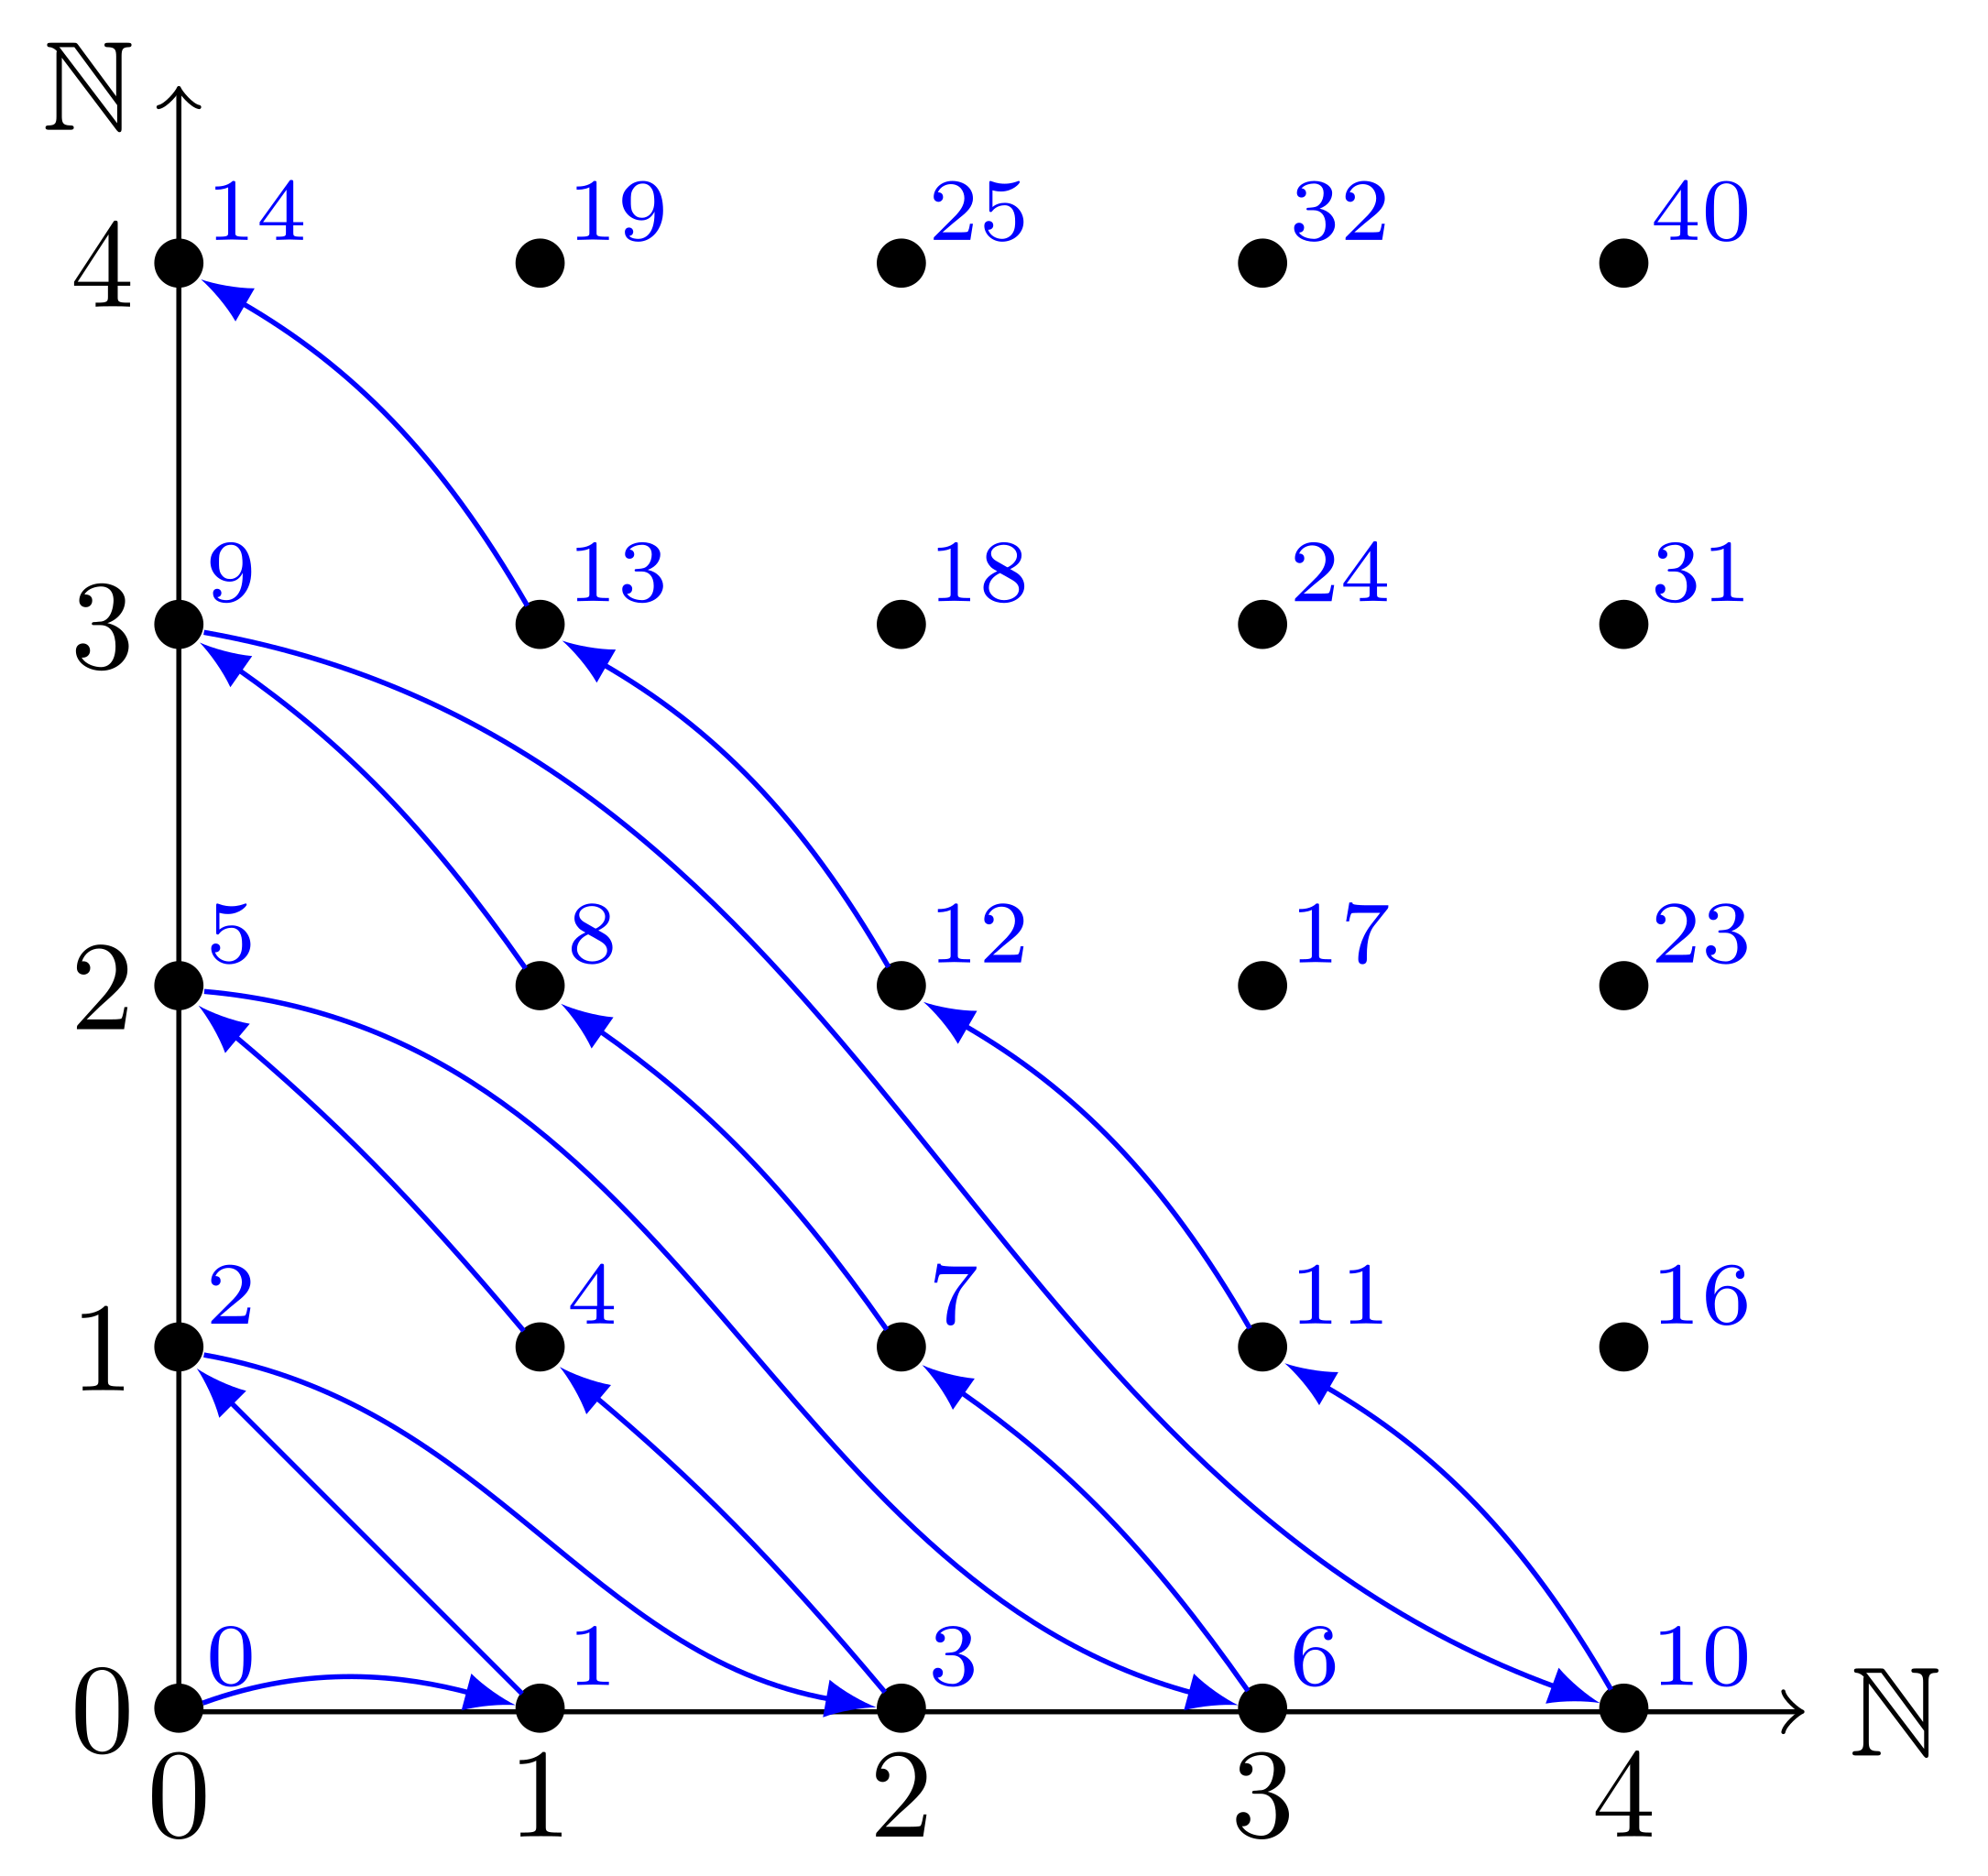
\includegraphics[width=0.35\textwidth]{Cantor}
  \label{fig:ejemplo}
\end{wrapfigure}

As we know $\N$ and $\N^2$ are isomorphic, we will use the ``Cantor Pairing Function'' $\pi$, which is a bijection between $\N$ and $\N^2$. Its expression is given by 
$$
\pi(k_1, k_2) = \dfrac{1}{2}(k_1 + k_2)(k_1 + k_2 + 1) + k_2;
$$

Thus, we tried to do a generalization of univariate multiple orthogonality where $|\vec n| = \pi(\exp(P_{\vec n}))$, instead of the degree of type I polynomial, where the function ``$\exp$'' represents the exponent of a polynomial (not the exponential function), \textit{i.e.}, if $$P(x,y)= c_{k} x^t y^s + c_{k-1} x^{t+1} y^{s-1} + \cdots c_2 y + c_1 x + c_0,$$ then $\exp(P)=(t,s)$ and $\pi(t,s)=k$.

Now, given $r\in\N$, $\vec n = (n_1,\dots, n_r)\in\N^r$ and a system of $r$ $2$-dimensional measures $\mu_1, \dots, \mu_r$, we are now presenting the definitions of type I and II multiple orthogonality following this approach. 

\begin{definition}[Type II Multiple Orthogonality]
  The \textbf{bivariate type II multiple orthogonal polynomial} $P_{\vec n}(x,y)$ is a monic polynomial such that $\exp(P_{\vec n})=\pi^{-1}(|\vec n|)$,  and satisfying
  \begin{equation}
    \label{eq:typeII-MOP-2-app}
    \boxed{
    \prodesc{P_{\vec n}}{x^t y^s}_j = 0, \ \ \ 0\leq \pi(t,s)\leq n_j-1, j=1,\dots,r.}
  \end{equation}    
\end{definition}

\begin{definition}
  \textbf{Bivariate type I multiple orthogonal polynomials} are often presented in a vector $(A_{\vec n,1}(x,y),\dots,A_{\vec n,r}(x,y))$ where $\exp(A_{\vec n,j}) \leq \pi^{-1}(n_j-1)$. This means, if $n_j-1 = \pi(t_j,s_j)$, then $A_{\vec n,j} = c_{n_j-1} x^{t_j}y^{s_j}+\cdots + c_0$. This polynomials satisfy
  \begin{equation}
    \label{eq:condition-type-I-2-app}
    \boxed{\sum_{j=1}^r \prodesc{A_{\vec n,j}}{x^t y^s}_j = \left\{\begin{array}{ccl}
        0 &   \text{ if } & 0\leq \pi(t,s)\leq |\vec n|-2 \\
        1 & \text{ if } & \pi(t,s)= |\vec n|-1     
    \end{array}\right.}.
  \end{equation}
\end{definition}

  As occurs in the first approach, Type II and Type I polynomials existence is equivalent.% For $\vec n=(n_1,\dots,n_r)$, type I and type II polynomials exist if, and only if the matrix
%
%  \begin{eqnarray}
%    M_{\vec n} = \begin{pmatrix}
%     M^{(1)} | \cdots | M^{(r)}
%    \end{pmatrix} , \text{ where } M^{(j)} = \begin{pmatrix}
%      m_{0,0}^{(1)} & \cdots & m_{\pi^{-1}(n_j-2)}^{(1)}  & m_{\pi^{-1}(n_j-1)}^{(1)}  \\
%      m_{1,0}^{(1)} & \cdots & m_{\pi^{-1}(n_j-2)+(1,0)}^{(1)}  & m_{\pi^{-1}(n_j-1)+(1,0)}^{(1)}  \\
%      \vdots & \ddots & \vdots & \vdots \\
%      m_{\pi^{-1}(|\vec n|-1)}^{(1)} & \cdots & m_{\pi^{-1}(n_j-2)+\pi^{-1}(|\vec n|-1)}^{(1)}  & m_{\pi^{-1}(n_j-1)+\pi^{-1}(|\vec n|-1)}^{(1)}  \\
%    \end{pmatrix}
%  \end{eqnarray}
%  

  With the first approach only a few multi-indices allowed us to create MOP vectors, whereas in this second approach it is possible to calculate bivariate MOP with any $\vec n\in\N^r$. Apart from that, the degree of the type II polynomials and the number of orthogonality conditions in type I orthogonality is exactly $|\vec n|$, just like happens in univariate multiple orthogonality. Nevertheless, the conditions \eqref{eq:typeII-MOP-2-app} and \eqref{eq:condition-type-I-2-app} are less intuitive than \eqref{eq:typeII-MOP-d-variables} and \eqref{eq:condition-type-ii} with respect to the original conditions \eqref{eq:typeII-MOP-dot} and \eqref{eq:typeI-MOP-dot}.


\vspace{2pt}

%%%%%%%%%%%%%%%%%%%%%%%%%%%%%%%%%%%%%%%%%%%%%%%%%%%%%%%%%%%%%%%%%%%%%%%%%%%%%%%
}
%%%%%%%%%%%%%%%%%%%%%%%%%%%%%%%%%%%%%%%%%%%%%%%%%%%%%%%%%%%%%%%%%%%%%%%%%%%%%%%
%
%%%%%%%%%%%%%%%%%%%%%%%%%%%%%%%%%%%%%%%%%%%%%%%%%%%%%%%%%%%%%%%%%%%%%%%%%%%%%%
%%%%%%%%%%%%%%%%%%%%%%%%%%%%%%%%%%%%%%%%%%%%%%%%%%%%%%%%%%%%%%%%%%%%%%%%%%%%%%
%%%%%%%%%%%%%%%%%%%%%%%%%%%%%%%%%%%%%%%%%%%%%%%%%%%%%%%%%%%%%%%%%%%%%%%%%%%%%%%


%%%%%%%%%%%%%%%%%%%%%%%%%%%%%%%%%%%%%%%%%%%%%%%%%%%%%%%%%%%%%%%%%%%%%%%%%%%%%%%
\headerbox{\ 5. Future research topics }{name=future,below=first,row=3,column=0,span=1}
{
%%%%%%%%%%%%%%%%%%%%%%%%%%%%%%%%%%%%%%%%%%%%%%%%%%%%%%%%%%%%%%%%%%%%%%%%%%%%%%
%\begin{multicols}{2}
  Multiple Orthogonal Polynomials is a theory that is currently being widely researched. At this moment, we have generalised to the bivariate case some of the main univariate results. But there are still many results and applications to work on:
  \begin{itemize}
    \item Study product of two univariate MOP $P_{\vec n}(x)P_{\vec m}(y)$ as a bivariate MOP. 
    \item Find Nearest Neighbour Relation generalizations to the bivariate case for general paths in both approaches.
    \item Find a possible connection between the two definitions.
    \item Look for applications to Hermite-Padé rational approximations and random matrices.
    \item Generalise existing examples to the bivariate case: Jacobi-Piñeiro, Jacobi-Angelesco, OP defined in the Simplex, etc.
    \item \dots
  \end{itemize}
%\end{multicols}


%%%%%%%%%%%%%%%%%%%%%%%%%%%%%%%%%%%%%%%%%%%%%%%%%%%%%%%%%%%%%%%%%%%%%%%%%%%%%%
}



































%
%
%%%%%%%%%%%%%%%%%%%%%%%%%%%%%%%%%%%%%%%%%%%%%%%%%%%%%%%%%%%%%%%%%%%%%%%%%%%%%%%
    \headerbox{\ References and Acknowledgements}{name=references,column=1,below=first}{
%%%%%%%%%%%%%%%%%%%%%%%%%%%%%%%%%%%%%%%%%%%%%%%%%%%%%%%%%%%%%%%%%%%%%%%%%%%%%%%

\smaller
\bibliographystyle{ieee}
\renewcommand{\section}[2]{\vskip 0.05em}
\begin{thebibliography}{1}\itemsep=-0.01em
\setlength{\baselineskip}{0.4em}
\bibitem{chiara}
{\sc T. S. Chiara},
{\em An Introduction to Orthogonal Polynomials},
{\rm Dover Books on Mathematics, Dover Publications, 2011}
\bibitem{xu}
{\sc C. F. Dunkl and Y. Xu},
{\em Orthogonal polynomials of several variables},
{\rm 2nd edition, Encyclopedia of Mathematics and its Applications, vol. 155, Cambridge Univ. Press, Cambridge, 2014.}
\bibitem{Walter}
{\sc W. van Assche},
{\em Orthogonal and multiple orthogonal polynomials, random matrices, and painlevé equations}, in 
{\rm ``Orthogonal Polynomials'' (M. Foupouagnigni, W. Koepf, eds), Tutorials, Schools and Workshops in the Mathematical Sciences, Springer Nature Switzerland} (2020) 629--683.
\bibitem{ismail}
{\sc M. E. H. Ismail},
{\em Classical and quantum orthogonal polynomials in one variable},
{\rm Cambridge University Press, Encyclopedia of mathematics and its applications}, 98, (2005).
\bibitem{3}
{\sc A. Martínez-Finkelshtein, W. van Assche},
{\em What is \dots a multiple orthogonal polynomial?},
{\rm Notices of the American Mathematical Society}, 63, (2016) 1029--1031.
\end{thebibliography}



{\noindent\hspace*{-5pt}
%\begin{tabular}{p{0.8\textwidth}p{0.15\textwidth}}
\noindent{\normalsize\textbf{Acknowledgements}} Universidad de Granada; GOYA: ``Grupo de Ortogonalidad Y Aplicaciones'' and ``Departamento de Matemática Aplicada''.}

\noindent Research supported by IMAG, María de Maeztu Grant ``IMAG CEX2020--001105--M''
\bigskip
%%& \hspace*{-5pt}
\vspace{1pt}
\centerline{

\includegraphics[height=1.1cm]{ugrH} \quad

\includegraphics[height=1.1cm]{IMAG} \quad

\includegraphics[height=1.1cm]{maeztu} \quad

\includegraphics[height=1.1cm]{goya.png}
}
%\end{tabular}

}
\end{poster}

\end{document} 